\paragraph{Results.} Validation selected $\gamma=\SimGamma$ (the largest value in the grid) and a GP length scale of \SimLengthscale\,d. On the \SimNEvents\ Nominal test events (\SimNModeled\ modelled, \SimNWithheld\ withheld), H1 \SimHOneVerdict, H2 and H3 \SimHTwoVerdict. Table~\ref{tab:sim} lists every strategy in every scenario.

\paragraph{H1, identification speed: refuted.} P reached a posterior of at least 0.95 on the true class after a median of \SimTtiP, and it got there for \SimIdP\ of modelled events (Fig.~\ref{fig:tti}). It was faster than the fixed cadence (which identified only \SimIdBzero), the auction baseline (median \SimTtiBone) and closed-world EIG (\SimTtiBthree; Holm $p$ \SimHolmBthree\ for each). But it was not faster than classifier-entropy sampling B2, whose median was \SimTtiBtwo. The paired test does favour P over B2 (Holm $p=\SimHolmBtwo$), but only because B2 identified just \SimIdBtwo\ of events, and unidentified events rank last. Looking pair by pair, P was slower in \SimSlowerBtwo\ of pairs and faster in \SimFasterBtwo. The preregistered criterion asks for a shorter median, so H1 fails. P also beats closed-world EIG here for an unflattering reason. Under causality, B3 greedily jumps to late, high-contrast epochs, so it uses only \SimObsAllBthree\ of its 5 measurements, against \SimObsAllP\ for P.

\begin{figure}[t]
\centering
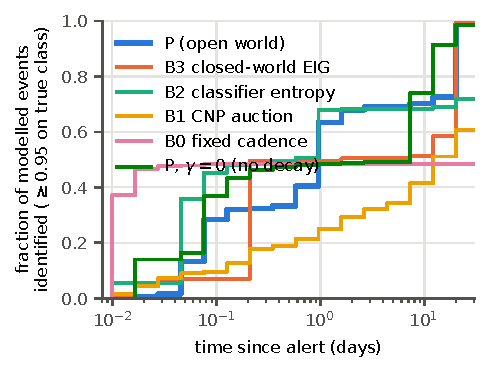
\includegraphics[width=\columnwidth]{generated/figures/fig1_tti.pdf}
\caption{H1. Cumulative fraction of modelled events whose posterior on the true class has reached 0.95, by time since alert (Nominal, test). B2 identifies the events it can identify earliest. P identifies almost all of them, but later. Closed-world EIG (B3) leaves many identifications to the final epochs.}
\label{fig:tti}
\end{figure}

\paragraph{H2, irreversibility: supported, with caveats.} Removing the decay term cut the information recovered about the true class's amplitude by \SimHtwoFast\ nats on fast classes and by \SimHtwoSlow\ on the slow GRB afterglow, a difference of \SimHtwoEst\ \SimHtwoCI. Kilonovae carry most of this effect (\SimDeltaKilonova), and shock cooling carries some of it (\SimDeltaShock). For the fastest class, the M-dwarf flare, the decay term actually lost information (\SimDeltaFlare; Fig.~\ref{fig:decay}). The effect also reversed under model error, because the wrong timescales mislead the urgency estimate (\SimHtwoModelErrorEst\ \SimHtwoModelErrorCI).

\begin{figure}[t]
\centering
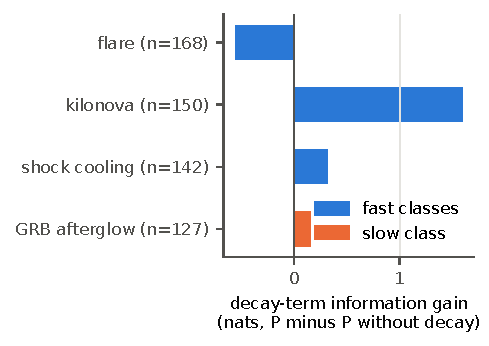
\includegraphics[width=\columnwidth]{generated/figures/fig2_decay.pdf}
\caption{H2. Information about the true amplitude gained from the decay term, per class (P minus P without it), Nominal test. The gain is positive for kilonova and shock cooling, near zero for the slow class, and negative for flares.}
\label{fig:decay}
\end{figure}

\paragraph{H3, open-world detection: supported.} At a 5\% false-alarm rate on modelled events, P's $P(h_0)$ detected \SimTprP\ of withheld events. A threshold on B3's closed-world posterior entropy detected \SimTprBthree\ (difference \SimHthreeEst\ points, 95\% CI \SimHthreeCI; Fig.~\ref{fig:rocsim}). The AUROC was \SimAucP\ for $P(h_0)$, against \SimAucBthree\ for B3 entropy and \SimAucBtwo\ for B2 entropy. Entropy computed on P's own measurements did no better (\SimAucPown), so the gain comes from the hypothesis itself and not from the measurements P chose. Without $h_0$, closed-world EIG was confidently wrong on \SimCwWhBthreeAll\ of withheld events, and P on \SimCwWhPAll. P made no false ``unknown'' calls on modelled events (\SimFaP) and kept the same modelled accuracy as B3 (\SimAccModPAll). H3 held in all three scenarios, but model error is the failure mode we predicted. Under model error, P called \SimFaPModelError\ of modelled events unknown, and its modelled accuracy fell to \SimAccModPModelError\ (B3: \SimAccModBthreeModelError).

\begin{figure}[t]
\centering
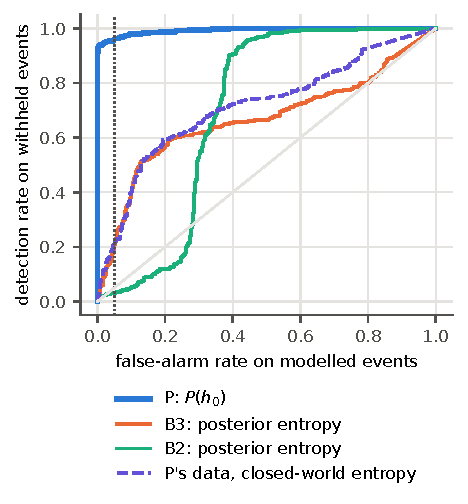
\includegraphics[width=\columnwidth]{generated/figures/fig3_roc_sim.pdf}
\caption{H3. ROC for separating withheld from modelled events (Nominal, test). The dotted line marks the preregistered 5\% false-alarm operating point.}
\label{fig:rocsim}
\end{figure}

\paragraph{Ablations.} Removing the adequacy term changed nothing we could measure. P$_{\beta=0}$ flagged \SimFlagNoAdeq\ of withheld events (P: \SimFlagP), with an AUROC of \SimAucAblNoAdeq\ (P: \SimAucAblP). Removing the decay term did matter. P$_{\gamma=0}$ took \SimObsAllNoDecay\ measurements instead of \SimObsAllP, flagged \SimFlagNoDecay, and was confidently wrong on \SimCwWhNoDecayAll\ of withheld events. So in this setting, the decay term helps open-world detection mainly by stopping the planner from spending its horizon too early, which leaves $h_0$ enough data to work with.

\begin{table*}[t]
\centering\scriptsize
\caption{Simulation test results (1000 events per scenario). Acc.\ mod.: accuracy on modelled events (\%). CW: confident-wrong rate (\%) on unmodelled (withheld) and modelled events. $\bar n_{\rm obs}$: measurements used, out of 5. Log score: mean log probability of the true outcome (closed-world strategies cannot express ``withheld'', so they are floored at $10^{-6}$).}
\label{tab:sim}
\begin{tabular}{llrrrrr}
\toprule
Scenario & Strategy & Acc.\ mod. & CW unmod. & CW mod. & $\bar n_{\rm obs}$ & log score \\
\midrule
Nominal & P (open world) & 100 & 6 & 0 & 4.2 & -0.19 \\
 & B3 closed-world EIG & 100 & 97 & 0 & 2.8 & -5.71 \\
 & B2 classifier entropy & 88 & 69 & 0 & 4.9 & -5.82 \\
 & B1 CNP auction & 80 & 75 & 0 & 3.2 & -5.92 \\
 & B0 fixed cadence & 79 & 1 & 0 & 5.0 & -5.92 \\
 & P, $\gamma=0$ (no decay) & 99 & 31 & 0 & 3.6 & -0.87 \\
 & P, $\beta=0$ (no adequacy) & 100 & 6 & 0 & 4.3 & -0.20 \\
\midrule
Crowding & P (open world) & 99 & 14 & 0 & 4.0 & -0.43 \\
 & B3 closed-world EIG & 100 & 94 & 0 & 3.0 & -5.82 \\
 & B2 classifier entropy & 94 & 80 & 0 & 4.8 & -5.88 \\
 & B1 CNP auction & 86 & 71 & 0 & 3.1 & -5.97 \\
 & B0 fixed cadence & 76 & 1 & 0 & 5.0 & -6.03 \\
 & P, $\gamma=0$ (no decay) & 100 & 31 & 0 & 3.4 & -0.96 \\
 & P, $\beta=0$ (no adequacy) & 99 & 14 & 0 & 4.1 & -0.43 \\
\midrule
Model error & P (open world) & 87 & 21 & 8 & 3.9 & -1.21 \\
 & B3 closed-world EIG & 99 & 96 & 1 & 2.9 & -6.11 \\
 & B2 classifier entropy & 81 & 29 & 4 & 5.0 & -6.32 \\
 & B1 CNP auction & 82 & 72 & 1 & 3.2 & -6.29 \\
 & B0 fixed cadence & 77 & 1 & 0 & 5.0 & -6.25 \\
 & P, $\gamma=0$ (no decay) & 93 & 26 & 6 & 3.4 & -1.32 \\
 & P, $\beta=0$ (no adequacy) & 86 & 21 & 8 & 3.9 & -1.21 \\
\bottomrule
\end{tabular}

\end{table*}

